\documentclass{article}

\usepackage[spanish]{babel}
\usepackage[utf8]{inputenc}
\usepackage{siunitx} % Provides the \SI{}{} and \si{} command for typesetting SI units
\usepackage{graphicx} % Required for the inclusion of images
\usepackage{amsmath} % Required for some math elements 
\usepackage{hyperref}
\usepackage{amsmath}
\usepackage{listings}
\usepackage{xcolor}
\usepackage{courier}
\usepackage[margin=1.2in]{geometry}
\usepackage{changepage}
\usepackage{titlesec}
\usepackage{wrapfig}
\usepackage{colortbl}
\usepackage{booktabs}
\usepackage{multirow}

\definecolor{codegreen}{rgb}{0,0.6,0}
\definecolor{codegray}{rgb}{0.5,0.5,0.5}
\definecolor{codepurple}{rgb}{0.58,0,0.82}
\definecolor{backcolour}{rgb}{0.95,0.95,0.92}

\lstdefinestyle{mystyle}{
    backgroundcolor=\color{backcolour},   
    commentstyle=\color{codegreen},
    keywordstyle=\color{magenta},
    numberstyle=\tiny\color{codegray},
    stringstyle=\color{codepurple},
    basicstyle=\ttfamily\footnotesize,
    breakatwhitespace=false,         
    captionpos=b,                    
    keepspaces=true,                 
    numbers=left,                    
    numbersep=5pt,                  
    showspaces=false,                
    showstringspaces=false,
    showtabs=false,                  
    tabsize=2
}
\lstset{language=Python, 
        basicstyle=\ttfamily\small, 
        keywordstyle=\color{keywords},
        commentstyle=\color{comments},
        stringstyle=\color{red},
        showstringspaces=false,
        identifierstyle=\color{codepurple},
        keywords=[2]{pow},
        keywordstyle=[2]{\color{orange}},
}

\lstset{style=mystyle}

\setlength\parindent{0pt} % Removes all indentation from paragraphs

\renewcommand{\labelenumi}{\alph{enumi}.} % Make numbering in the enumerate environment by letter rather than number (e.g. section 6)

\title{\textbf{Errores estadísticos y \\ determinación de la gravedad \\ con un péndulo simple}} % Title

\author{Víctor Mira Ramírez} % Author name

\date{\today} % Date for the report

\begin{document}

\maketitle % Insert the title, author and date

\begin{center}
\begin{tabular}{l r}

Profesora: & Carlos Sabater Piqueres\\
Grupo: & Grupo III \\
Lugar: & Universidad de Alicante
\end{tabular}
\end{center}

\tableofcontents

%----------------------------------------------------------------------------------------
%	SECTION 1
%----------------------------------------------------------------------------------------

\begin{abstract}
Este experimento tiene como objetivo estudia el movimiento de un péndulo simple para conseguir determinar la aceleración gravitatoria de en La Tierra. Se discutirá el tratamiento estadístico de medidas experimentales y cómo reducir el error en la medida.
\end{abstract}
\pagebreak

\section{Introducción}
Con el material suministrado para esta práctica se deberán medir las oscilaciones de un péndulo. La determinación
del periodo del péndulo tendrá un error elevado proveniente del observador. Estudiaremos la
influencia de dicho error en la medida y la forma de reducirlo. Finalmente obtenderemos un valor para la aceleración gravitatoria gracias a la relación que existe entre el periodo de oscilación y la longitud de la cuerda que sujeta al péndulo. Para todos estos cálculos necesitaremos usar una serie de ecuaciones:

\begin{equation}\label{eq:derivadas parciales}
    \centering
    \triangle{V} = \sqrt{\left(\frac{\partial{V}}{\partial{x}}\right)^2 \triangle{x}^2 + \left(\frac{\partial{V}}{\partial{y}}\right)^2 \triangle{y}^2 + \left(\frac{\partial{V}}{\partial{z}}\right)^2 \triangle{z}^2 }
\end{equation}

\vspace{0.3cm}

\begin{equation}\label{eq:graf}
    \centering
    y = a\cdot{x} + b
\end{equation}

\vspace{0.3cm}

\begin{equation}\label{eq:minscuad}
    \centering
    a_0 = \frac{N\sum x_i\cdot{y_i} - \sum x_i\cdot{y_i}}{N\sum {x_i}^2 - \left(\sum x_i \right)^2} \quad \Rightarrow \quad
    b_0 = \frac{\left(\sum x_i \right)^2\cdot{y_i} - \sum x_i\cdot\sum x_i\cdot{y_i}}{N\sum {x_i}^2 - \left(\sum x_i \right)^2}
\end{equation}

\vspace{0.3cm}

\begin{equation}\label{eq:errorminscuad}
    \centering
    \sigma_a = \sqrt{\frac{{\chi_N}^2}{N\cdot{Var(x)}}}
    \quad \Rightarrow \quad
    \sigma_b = \sqrt{\frac{{\chi_N}^2\cdot{\sum_(i=1)^(N) {x_i}^2}}{N\cdot{Var(x)}}}
\end{equation}

\begin{equation}\label{eq:relacion}
    \centering
    T = 2\pi \sqrt{\frac{l}{g}} \quad \Rightarrow \quad g = \frac{l}{\left( \frac{T}{2\pi}\right)^2}
\end{equation}

\vspace{0.3cm}

La ecuación \eqref{eq:derivadas parciales} se usará para la obtención del error de la gravedad respecto al error de la longitud y del periodo. Y \eqref{eq:graf} nos será útil una vez linealizada la gráfica, donde a es la pendiente y b la ordenada en el origen. Por último, la ecuación \eqref{eq:minscuad} es la de ajustes por mínimos cuadrados, útil para linealizar, junto con sus errores \eqref{eq:errorminscuad}. Por último, la ecuación \eqref{eq:relacion} nos servirá para relacionar la aceleración gravitatoria con las medidas ya obtenidas.

\section{Diagramas y formulaciones matemáticas}

El siguiente diagrama muestra un péndulo simple y las fuerzas que actúan sobre él. Podemos descomponer el peso en una componente radial ($P_{r} = m g \cos(\theta) $) y en una componente tangencial ($P_{t} = m g \sin(\theta) $)

\begin{figure}[h]
\centering
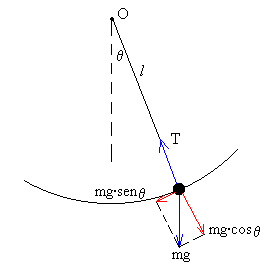
\includegraphics[width=.35\textwidth]{fotos/diagrama.png}
\end{figure}

Estudiamos el caso tanto en sentido radial, $ T - m g \cos(\theta) = m a_{c} = m l \omega^{2}$, donde $a_{c}$ es la aceleración centrípeta ($\frac{v^{2}}{r}$), quedándonos la ecuación para la Tensión: \[ \boxed{T = m g \cos(\theta) + m l \omega^{2}}\] y el caso en sentido tangencial, $ -m g \sin(\theta) = m a_{t} = m l \alpha = m l \frac{d^{2}\theta}{dt^{2}}$, donde $a_{t}$ es la aceleración tangencial ($\frac{dv}{dt}$), quedándonos la ecuación para el ángulo: \[\boxed{\frac{d^{2}\theta}{dt^{2}} + \frac{g}{l} \sin(\theta) = 0}\] \\\\ Con esta ecuación diferencial, conseguimos el ángulo en función al tiempo, $ \omega(t)$, a partir de la cual podemos averiguar la velocidad angular, $\omega(t) = \frac{d\theta}{dt}$ y la aceleración angular $\alpha(t) = \frac{d^{2}\theta}{dt^{2}}$

Resolver esta ecuación diferencial es algo complicado, pero existe un método rápido para obtener soluciones para ángulos pequeños detallada en el Anexo 1. En el Anexo 2 se detalla la evolución de la energía mecánica para nuestro péndulo.

\subsection{Solución Numérica}
Discretizando el tiempo y usando el método de Euler para pasos de $\Delta t$ pequeños, \\
$\omega = \frac{d\theta}{dt}\ \ \longrightarrow\ \ \ \frac{d^{2}\theta}{dt^{2}} + \frac{g}{l}\sin(\theta) = 0\ \ \longrightarrow\ \ \ \frac{d\omega}{dt} + \frac{g}{l}\sin(\theta) = 0\ \ \longrightarrow\ \ \ \Delta\omega = \left[ \frac{-g}{l}\sin(\theta)\right] \Delta t$ \\
y por tanto, obtenemos para la velocidad angular la ecuación: \[ \boxed{\omega_{i+1} = \omega_{i} - \left(\frac{g}{l}\sin(\theta_{i})\right)\Delta t}\] 
\\ y como $\omega = \frac{d\theta}{dt}\ \ \rightarrow\ \ \Delta \theta = \omega \Delta t$, obtenemos para el ángulo la ecuación: \[ \boxed{\theta_{i+1} = \theta_{i} + \omega_{i} \Delta t}\]

\subsection{Péndulo con Fricción}
La fuerza de rozamiento viene definida por la ecuación $F_{r} = -k \omega$, que debemos agregar a nuestra ecuación diferencial inicial, quedándonos la nueva ecuación diferencial: \[ -m g \sin(\theta) - k \omega = m l \alpha = m l \frac{d^2\theta}{dt^2} \] \[\boxed{\frac{d^{2}\theta}{dt^{2}} + \frac{g}{l} \sin(\theta) - \frac{k}{m l} \frac{d\theta}{dt} = 0}\]
Simplemente hemos añadido el término $- \frac{k}{m l} \frac{d\theta}{dt} = 0$ a nuestra ecuación diferencial.\\ \\
Actualizando nuestra solución numérica tenemos las siguientes ecuaciones para el caso con rozamiento:
\[ \boxed{\omega_{i+1} = \omega_{i} + \left[ \frac{-g}{l} \sin(\theta_{i}) + \frac{k}{m l}\omega_{i} \right] \Delta t}\]
\[ \boxed{\theta_{i+1} = \theta_{i} + \omega_{i} \Delta t}\]

%----------------------------------------------------------------------------------------
%	SECTION 4
%----------------------------------------------------------------------------------------

\section{Desarrollo experimental}
\subsection{Medición y Tratamiento Estadístico}
Primeramente, calculamos el periodo de un péndulo cuando la amplitud es pequeña y oscila 2 veces. Repetimos esta operación 20 veces, obtenemos el valor medio y la dispersión del periodo. \\\\ 
Ahora repetiremos el procedimiento seguido, pero esta vez haremos la medición una vez el péndulo haya oscilado 20 veces. Finalmente compararemos los valores obtenidos junto con la dispersión de los mismos. \\\\
Se realizará una representación de las distribuciones de los datos para cada uno de los casos anteriores. Se comprobará que el error estadístico en el segundo caso será mucho menor al primero.

\subsection{Cálculo de la aceleración gravitatoria y su error}
Con los datos obtenidos en la medición del apartado anterior, calcularemos la aceleración gravitatoria en La Tierra. Representaremos la dependencia del periodo de oscilación con la longitud del hilo, siendo la pendiente la aceleración gravitatoria. Discutiremos porqué se obtiene un valor para la odenada en el origen.  

\subsection{Medidas}
\begin{table}[htbp]
  \centering
  \hfill \break \\
    \begin{tabular}{|cccc|}
    \toprule
    \rowcolor[rgb]{ .357,  .608,  .835} \multicolumn{1}{|p{8em}}{\textcolor[rgb]{ 1,  1,  1}{t ± 0.25s, n = 2 }} & \multicolumn{1}{p{8em}}{\textcolor[rgb]{ 1,  1,  1}{t ± 0.25s,  n = 20  }} & \multicolumn{1}{p{8em}}{\textcolor[rgb]{ 1,  1,  1}{T ± 0.13s, n = 2  }} & \multicolumn{1}{p{8em}|}{\textcolor[rgb]{ 1,  1,  1}{T ± 0.013s, n = 20 }} \\
    \midrule
    \rowcolor[rgb]{ .608,  .761,  .902} \multicolumn{1}{|c|}{2,03} & \multicolumn{1}{c|}{\cellcolor[rgb]{ .741,  .843,  .933}21,89} & \multicolumn{1}{c|}{1,02} & \cellcolor[rgb]{ .741,  .843,  .933}1,095 \\
    \multicolumn{1}{|c|}{1,96} & \multicolumn{1}{c|}{21,89} & \multicolumn{1}{c|}{0,98} & 1,095 \\
    \rowcolor[rgb]{ .608,  .761,  .902} \multicolumn{1}{|c|}{2,14} & \multicolumn{1}{c|}{\cellcolor[rgb]{ .741,  .843,  .933}21,93} & \multicolumn{1}{c|}{1,07} & \cellcolor[rgb]{ .741,  .843,  .933}1,097 \\
    \multicolumn{1}{|c|}{2,03} & \multicolumn{1}{c|}{21,90} & \multicolumn{1}{c|}{1,02} & 1,095 \\
    \rowcolor[rgb]{ .608,  .761,  .902} \multicolumn{1}{|c|}{2,01} & \multicolumn{1}{c|}{\cellcolor[rgb]{ .741,  .843,  .933}21,96} & \multicolumn{1}{c|}{1,01} & \cellcolor[rgb]{ .741,  .843,  .933}1,098 \\
    \multicolumn{1}{|c|}{2,03} & \multicolumn{1}{c|}{21,95} & \multicolumn{1}{c|}{1,02} & 1,098 \\
    \rowcolor[rgb]{ .608,  .761,  .902} \multicolumn{1}{|c|}{2,01} & \multicolumn{1}{c|}{\cellcolor[rgb]{ .741,  .843,  .933}21,87} & \multicolumn{1}{c|}{1,01} & \cellcolor[rgb]{ .741,  .843,  .933}1,094 \\
    \multicolumn{1}{|c|}{2,01} & \multicolumn{1}{c|}{21,84} & \multicolumn{1}{c|}{1,01} & 1,092 \\
    \rowcolor[rgb]{ .608,  .761,  .902} \multicolumn{1}{|c|}{2,09} & \multicolumn{1}{c|}{\cellcolor[rgb]{ .741,  .843,  .933}21,83} & \multicolumn{1}{c|}{1,05} & \cellcolor[rgb]{ .741,  .843,  .933}1,092 \\
    \multicolumn{1}{|c|}{1,88} & \multicolumn{1}{c|}{21,83} & \multicolumn{1}{c|}{0,94} & 1,092 \\
    \rowcolor[rgb]{ .608,  .761,  .902} \multicolumn{1}{|c|}{2,02} & \multicolumn{1}{c|}{\cellcolor[rgb]{ .741,  .843,  .933}21,90} & \multicolumn{1}{c|}{1,01} & \cellcolor[rgb]{ .741,  .843,  .933}1,095 \\
    \multicolumn{1}{|c|}{2,00} & \multicolumn{1}{c|}{22,08} & \multicolumn{1}{c|}{1,00} & 1,104 \\
    \rowcolor[rgb]{ .608,  .761,  .902} \multicolumn{1}{|c|}{2,02} & \multicolumn{1}{c|}{\cellcolor[rgb]{ .741,  .843,  .933}21,95} & \multicolumn{1}{c|}{1,01} & \cellcolor[rgb]{ .741,  .843,  .933}1,098 \\
    \multicolumn{1}{|c|}{2,02} & \multicolumn{1}{c|}{21,90} & \multicolumn{1}{c|}{1,01} & 1,095 \\
    \rowcolor[rgb]{ .608,  .761,  .902} \multicolumn{1}{|c|}{2,06} & \multicolumn{1}{c|}{\cellcolor[rgb]{ .741,  .843,  .933}22,02} & \multicolumn{1}{c|}{1,03} & \cellcolor[rgb]{ .741,  .843,  .933}1,101 \\
    \multicolumn{1}{|c|}{2,00} & \multicolumn{1}{c|}{21,94} & \multicolumn{1}{c|}{1,00} & 1,097 \\
    \rowcolor[rgb]{ .608,  .761,  .902} \multicolumn{1}{|c|}{2,02} & \multicolumn{1}{c|}{\cellcolor[rgb]{ .741,  .843,  .933}21,96} & \multicolumn{1}{c|}{1,01} & \cellcolor[rgb]{ .741,  .843,  .933}1,098 \\
    \multicolumn{1}{|c|}{2,13} & \multicolumn{1}{c|}{21,84} & \multicolumn{1}{c|}{1,07} & 1,092 \\
    \rowcolor[rgb]{ .608,  .761,  .902} \multicolumn{1}{|c|}{2,07} & \multicolumn{1}{c|}{\cellcolor[rgb]{ .741,  .843,  .933}22,01} & \multicolumn{1}{c|}{1,04} & \cellcolor[rgb]{ .741,  .843,  .933}1,101 \\
    \multicolumn{1}{|c|}{1,94} & \multicolumn{1}{c|}{21,88} & \multicolumn{1}{c|}{0,97} & 1,094 \\
    \midrule
    \midrule
    \rowcolor[rgb]{ 1,  .902,  .6} 2,02  & 21,92 & 1,01  & 1,096 \\
    \bottomrule
    \end{tabular}%
  \label{tab:addlabel}%
\end{table}%

La fila resaltada en amarillo refleja la media de los datos de la columna bajo la que se encuentre el valor.

\paragraph{Material proporcionado}\mbox{}
    \begin{tabular}{ll}
        Hilo para péndulo& \\
        Bola para péndulo& \\
        Cinta métrica    & \\
        Cronómetro       & \\
    \end{tabular}    
    
\paragraph{Otras medidas}\mbox{}
    \begin{tabular}{ll}
        Longitud del hilo& $0.3\,\pm\  0.1\,m$\\
    \end{tabular}    

\section{Resultados y Discusiones}
\subsection{Tratamiento Estadísico}
El valor medio del periodo para n = 2 oscilaciones fue de 1.01 segundos, con una dispersión de 0.03 segundos, y por tanto un error estadístico de 0.007 segundos. \\\\
Sin embargo para n = 20 oscilaciones, el periodo medio fue de 1.093 segundos, obtenemos una dispersión de 0.003 segundos, y un error estadístico de 0.0007 segundos. ¡Un orden de magnitud menor! \\\\Esto se debe a que en dos oscilaciones el error de interacción será muy grande relativo al tiempo que el péndulo está oscilando. Este error se reduce en porcentaje cuando aumentamos las oscilaciones, y por tanto el tiempo total que está oscilando el péndulo

\begin{figure}[h]
\centering
\hspace*{-2.2cm}
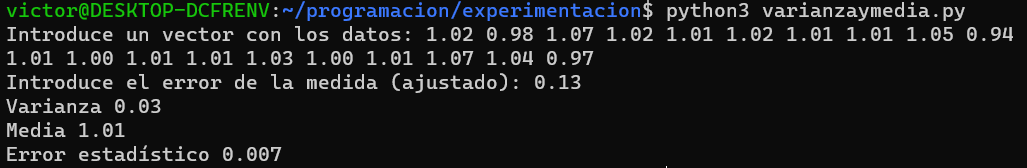
\includegraphics[width=.56\textwidth]{fotos/ErrEst2corto.png}\hfill
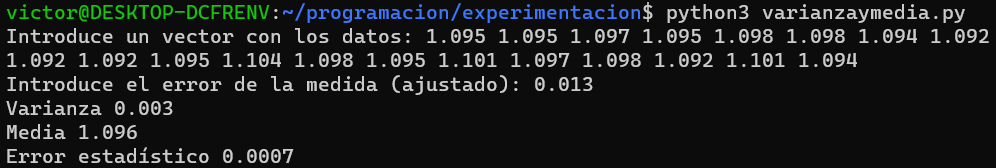
\includegraphics[width=.56\textwidth]{fotos/ErrEst20corto.png}
\hspace*{-2.2cm}
\end{figure}

El error de la medida (0.13s y 0.013s respectivamente) fue calculado usando propagación de errores desde el error del tiempo que tardó en realizar las n oscilaciones (0.25 segundos). \\
$\Delta T_{n=2} = \sqrt{\left( \frac{\partial{T}}{\partial{t}}\right)^2\left(\Delta t\right)^2} \quad = \quad \sqrt{\left(\frac{t}{2}\right)^2\left(\Delta t\right)^2}  \quad = \quad \sqrt{0.5^2 \cdot 0.25^2} \quad = \quad 0.13s$ \\\\
$\Delta T_{n=20} = \sqrt{\left( \frac{\partial{T}}{\partial{t}}\right)^2\left(\Delta t\right)^2} \quad = \quad \sqrt{\left(\frac{t}{20}\right)^2\left(\Delta t\right)^2}  \quad = \quad \sqrt{0.05^2 \cdot 0.25^2} \quad = \quad 0.013s$ 
\\\\
En la siguiente figura vemos representados las dos columnas del periodo, donde la curva naranja es el periodo calculado para n = 20, y la curva azul para n = 2. Podemos comprobar como la curva naranja es mucho menos dispersa que la azul, que tiene muchos más picos.

\begin{figure}
    \centering
    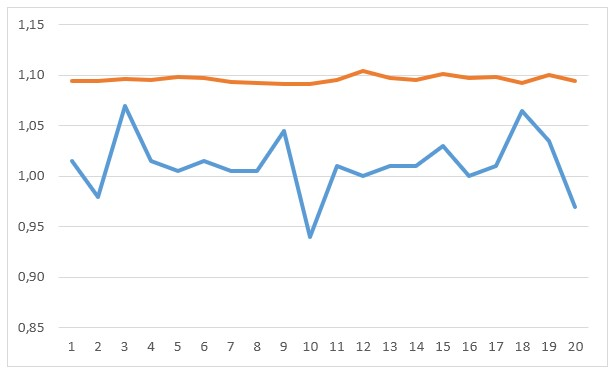
\includegraphics[width=.45\textwidth]{fotos/periodo.jpg}
    \caption{Periodo para 20 oscilaciones}
\end{figure}
Para los futuros cálculos usaremos únicamente el valor del periodo para n = 20, que sabemos que nos dará una mayor precisión. \\
Después de añadir el respectivo error de interacción (0.3s) y del cronómetro (0.01s), obtenemos un valor final para el periodo de 1.10 ± 0.02s
\subsection{Cálculo de la gravedad}
Una vez obtenido el periodo y su error, procedemos a calcular la aceleración gravitatoria usando la fórmula que la relaciona con la longitud del hilo y el periodo. \\\\ Calculamos mediante propagación de errores y el uso de las derivadas parciales el error para la aceleración gravitatoria. \\\\ Obtenemos como valor final una aceleración gravitatoria de 9.8 ± 0.4 m/s²
\begin{figure}[h]
    \centering
    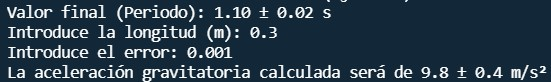
\includegraphics[width=.6\textwidth]{fotos/gravedad.jpg}
    \caption{Aceleración Gravitatoria}
\end{figure}
\subsubsection{Linealización}
Aquí iría la linealización para n = 20 constante y diferentes longitudes. Se obtiene como pendiente la gravedad y se muestra el gráfico. No he tenido tiempo de acabarlo pero este es el hueco para ello.

%----------------------------------------------------------------------------------------
%	SECTION 5
%----------------------------------------------------------------------------------------

\pagebreak
\section{Anexo}
\subsection{Formulación de ángulos pequeños - Anexo 1}
    La ecuación $\frac{d^{2}\theta}{dt^{2}} + \frac{g}{l} \sin(\theta) = 0$ puede simplificarse si, considerando ángulos pequeños, $\sin(\theta) = 0$, obteniendo la fórmula $\frac{d^{2}\theta}{dt^{2}} + \frac{g}{l} \theta) = 0$, que tiene una solución exacta, \[ \boxed{\theta = \theta_0 \cos(\gamma t)\ \ \ \ \ \ \ \theta_0 = \theta (t = 0)}\] donde $\gamma$ es la frecuencia angular, $\gamma^{2} = \frac{g}{l} \ \ \longrightarrow\ \ \ \gamma = \sqrt{\frac{g}{l}}$\\\\
    y como $\omega = \frac{d\theta}{dt}$: \[\boxed{\omega = \theta_0 \gamma \left(-\sin(\gamma t)\right)} \]

\subsection{Energías - Anexo 2}
    Trivialmente sabemos que la Energía Mecánica será la suma de la Energía Potencial y de la Energía Cinética. En el caso sin rozamiento, habrá una conservación de la Energía Mecánica, ya que no existirá ninguna energía disipatoria que la reduzca. Ese es el caso con rozamiento, donde el rozamiento irá poco a poco reduciendo nuestra energía mecánica total hasta llegar al punto donde no oscilará.
        \paragraph{Energía Potencial}\mbox{}\\\\
            Sabiendo que la fórmula de la Energía Potencial es $E_{p} = -m g h$ y que la altura del péndulo en cada momento viene dada por $\cos(\theta)l$, obtenemos para la Energía Potencial de nuestro péndulo la ecuación: \\\[ \boxed{E_{p} = -m g l \cos(\theta)}\]
        \paragraph{Energía Cinética}\mbox{}\\\\
            Sabiendo que la fórmula de la Energía Cinética es $E_{c} = \frac{1}{2} m v^2$ y que la velocidad tangencial se relaciona con la angular con la fórmula $v = \omega r$, donde $r$ será la longitud de la cuerda del péndulo $l$, obtenemos para la Energía Cinética de nuestro péndulo la ecuación \\\[ \boxed{E_{c} = \frac{1}{2} m \omega^{2} l^{2}}\]


\paragraph{Gráficas}\mbox{}

\begin{figure}[h]
\begin{wrapfigure}{l}{0.55\textwidth}
\centering
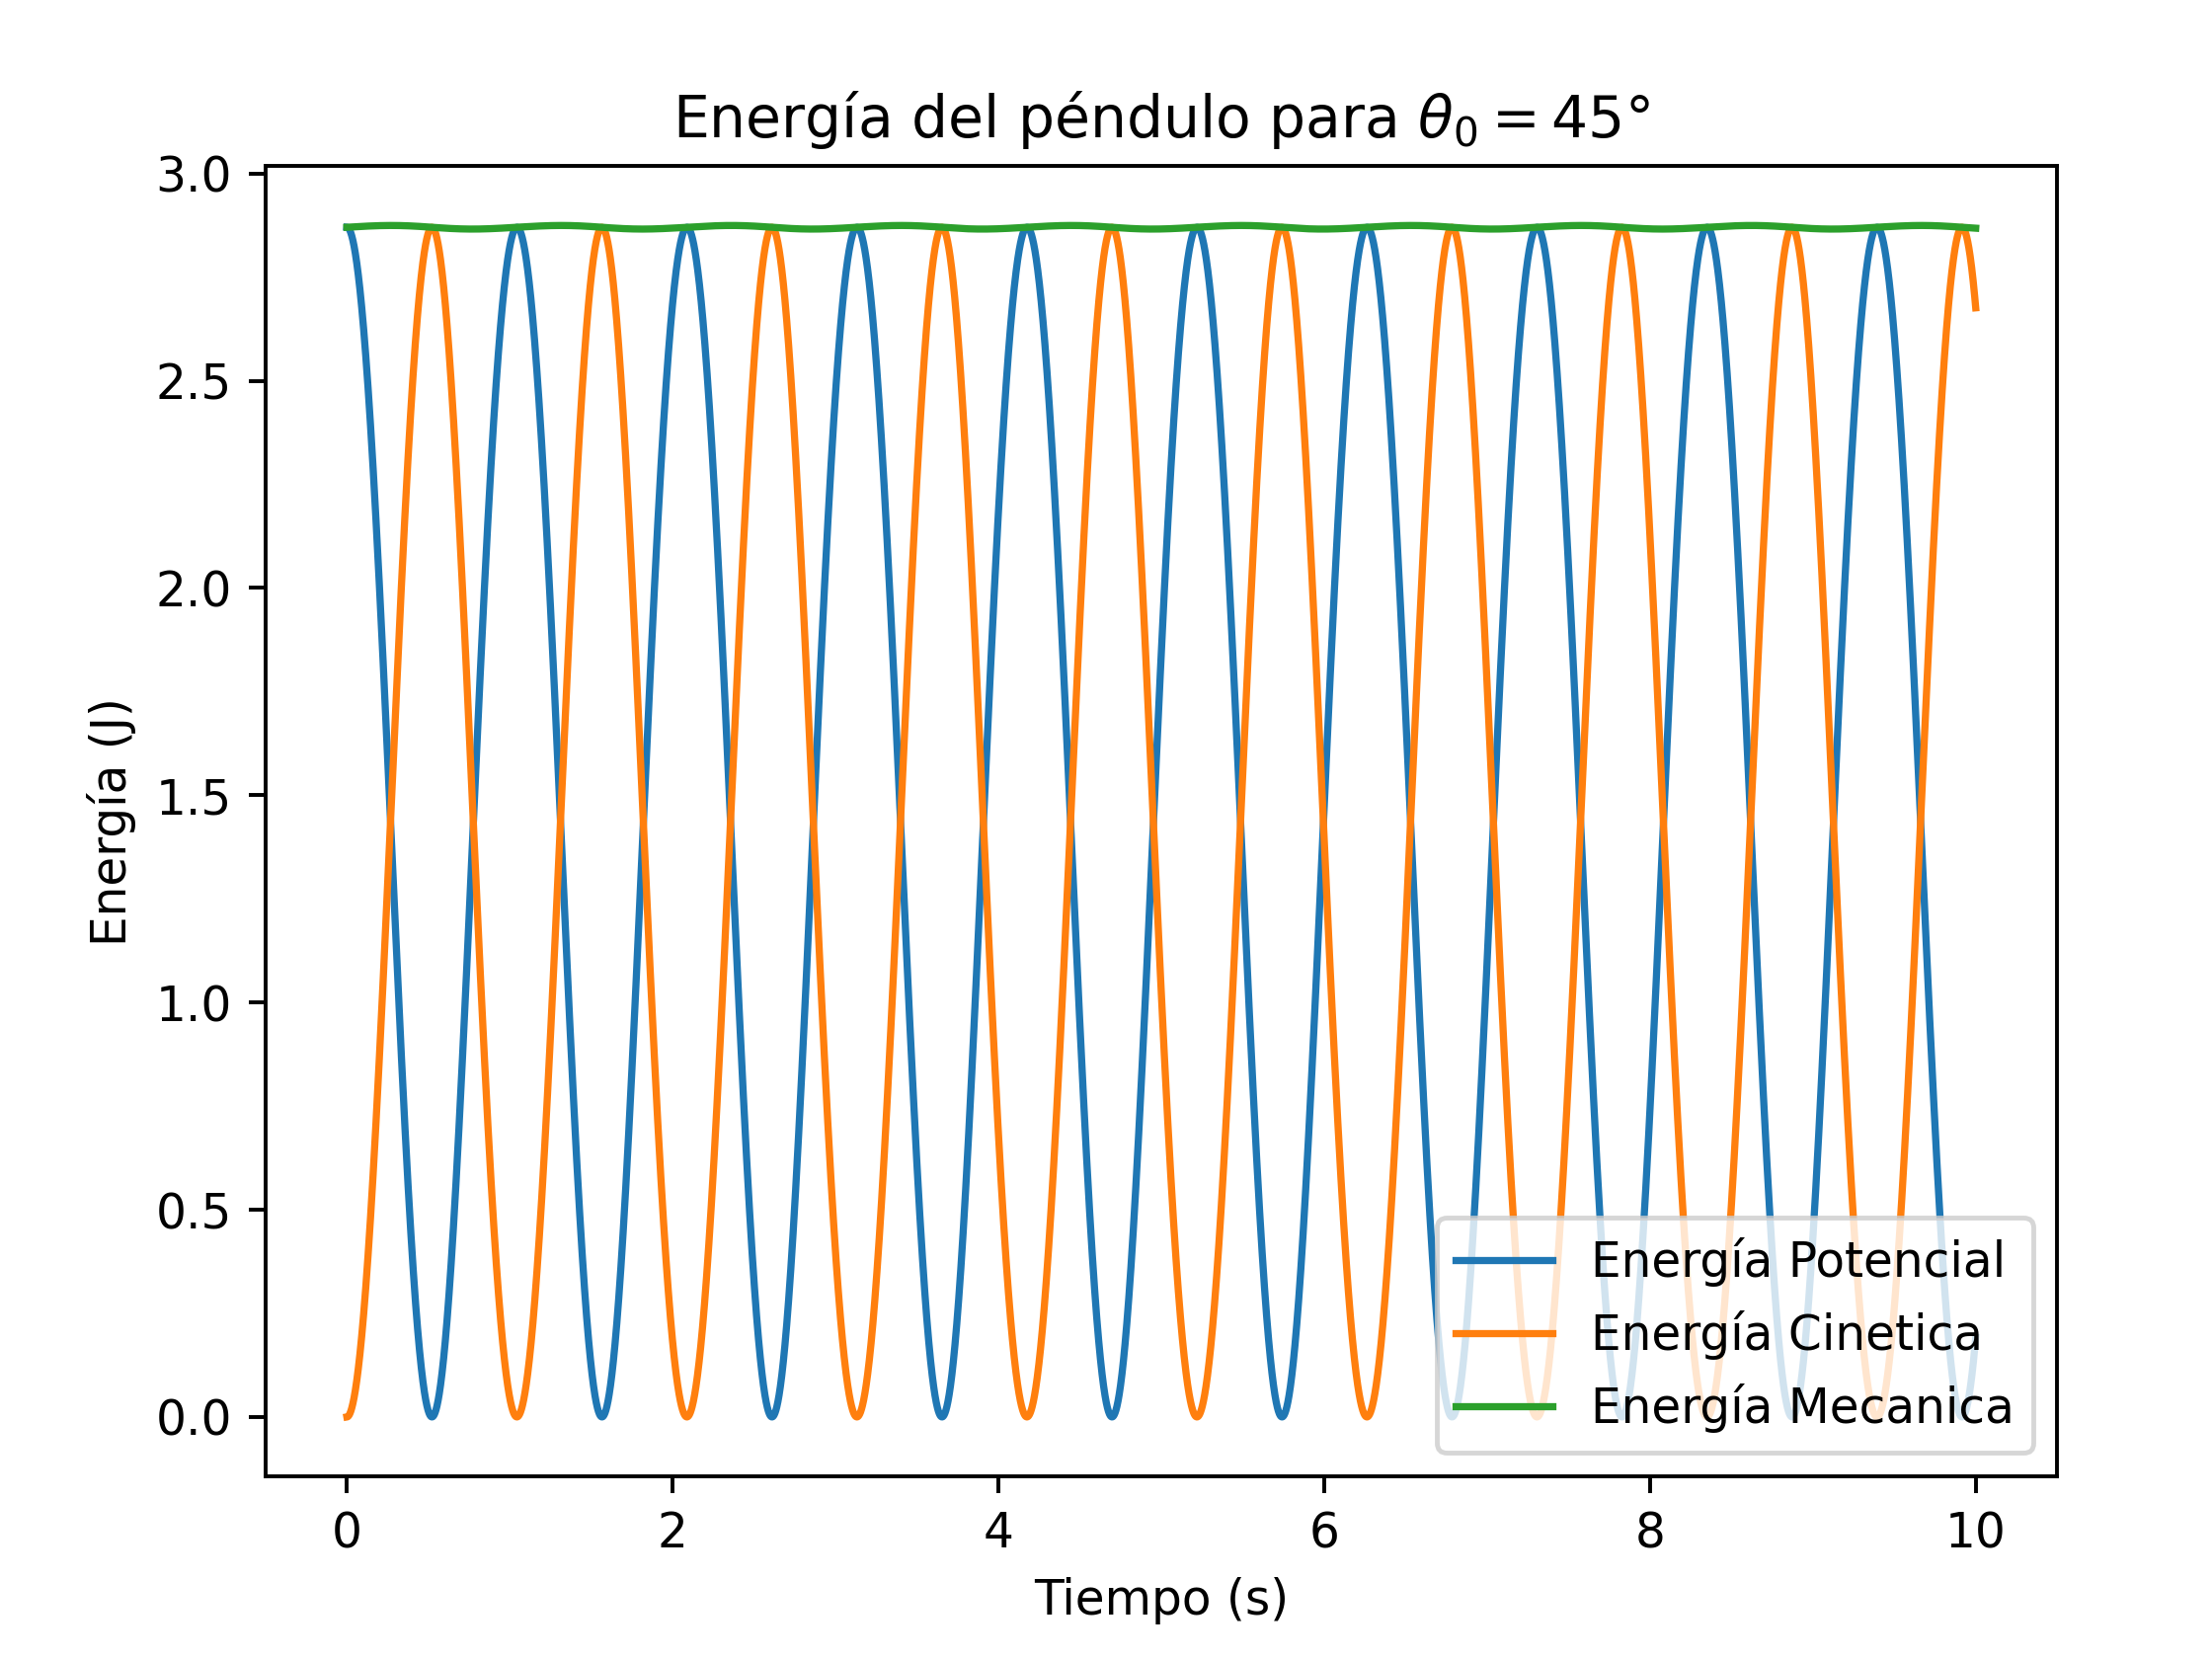
\includegraphics[width=.55\textwidth]{fotos/Fig5.png}
\end{wrapfigure}
\hfill \break \\\\
Esta es la gráfica de las energías del péndulo en función al tiempo para un péndulo soltado desde 45 grados. Esta gráfica ha sido calculada usando el método que no tiene en cuenta el rozamiento, lo cual refleja una conservación de la energía mecánica, que es constante.
\end{figure}

\hfill \break \\

\begin{figure}[h]
\begin{wrapfigure}{l}{0.55\textwidth}
\centering
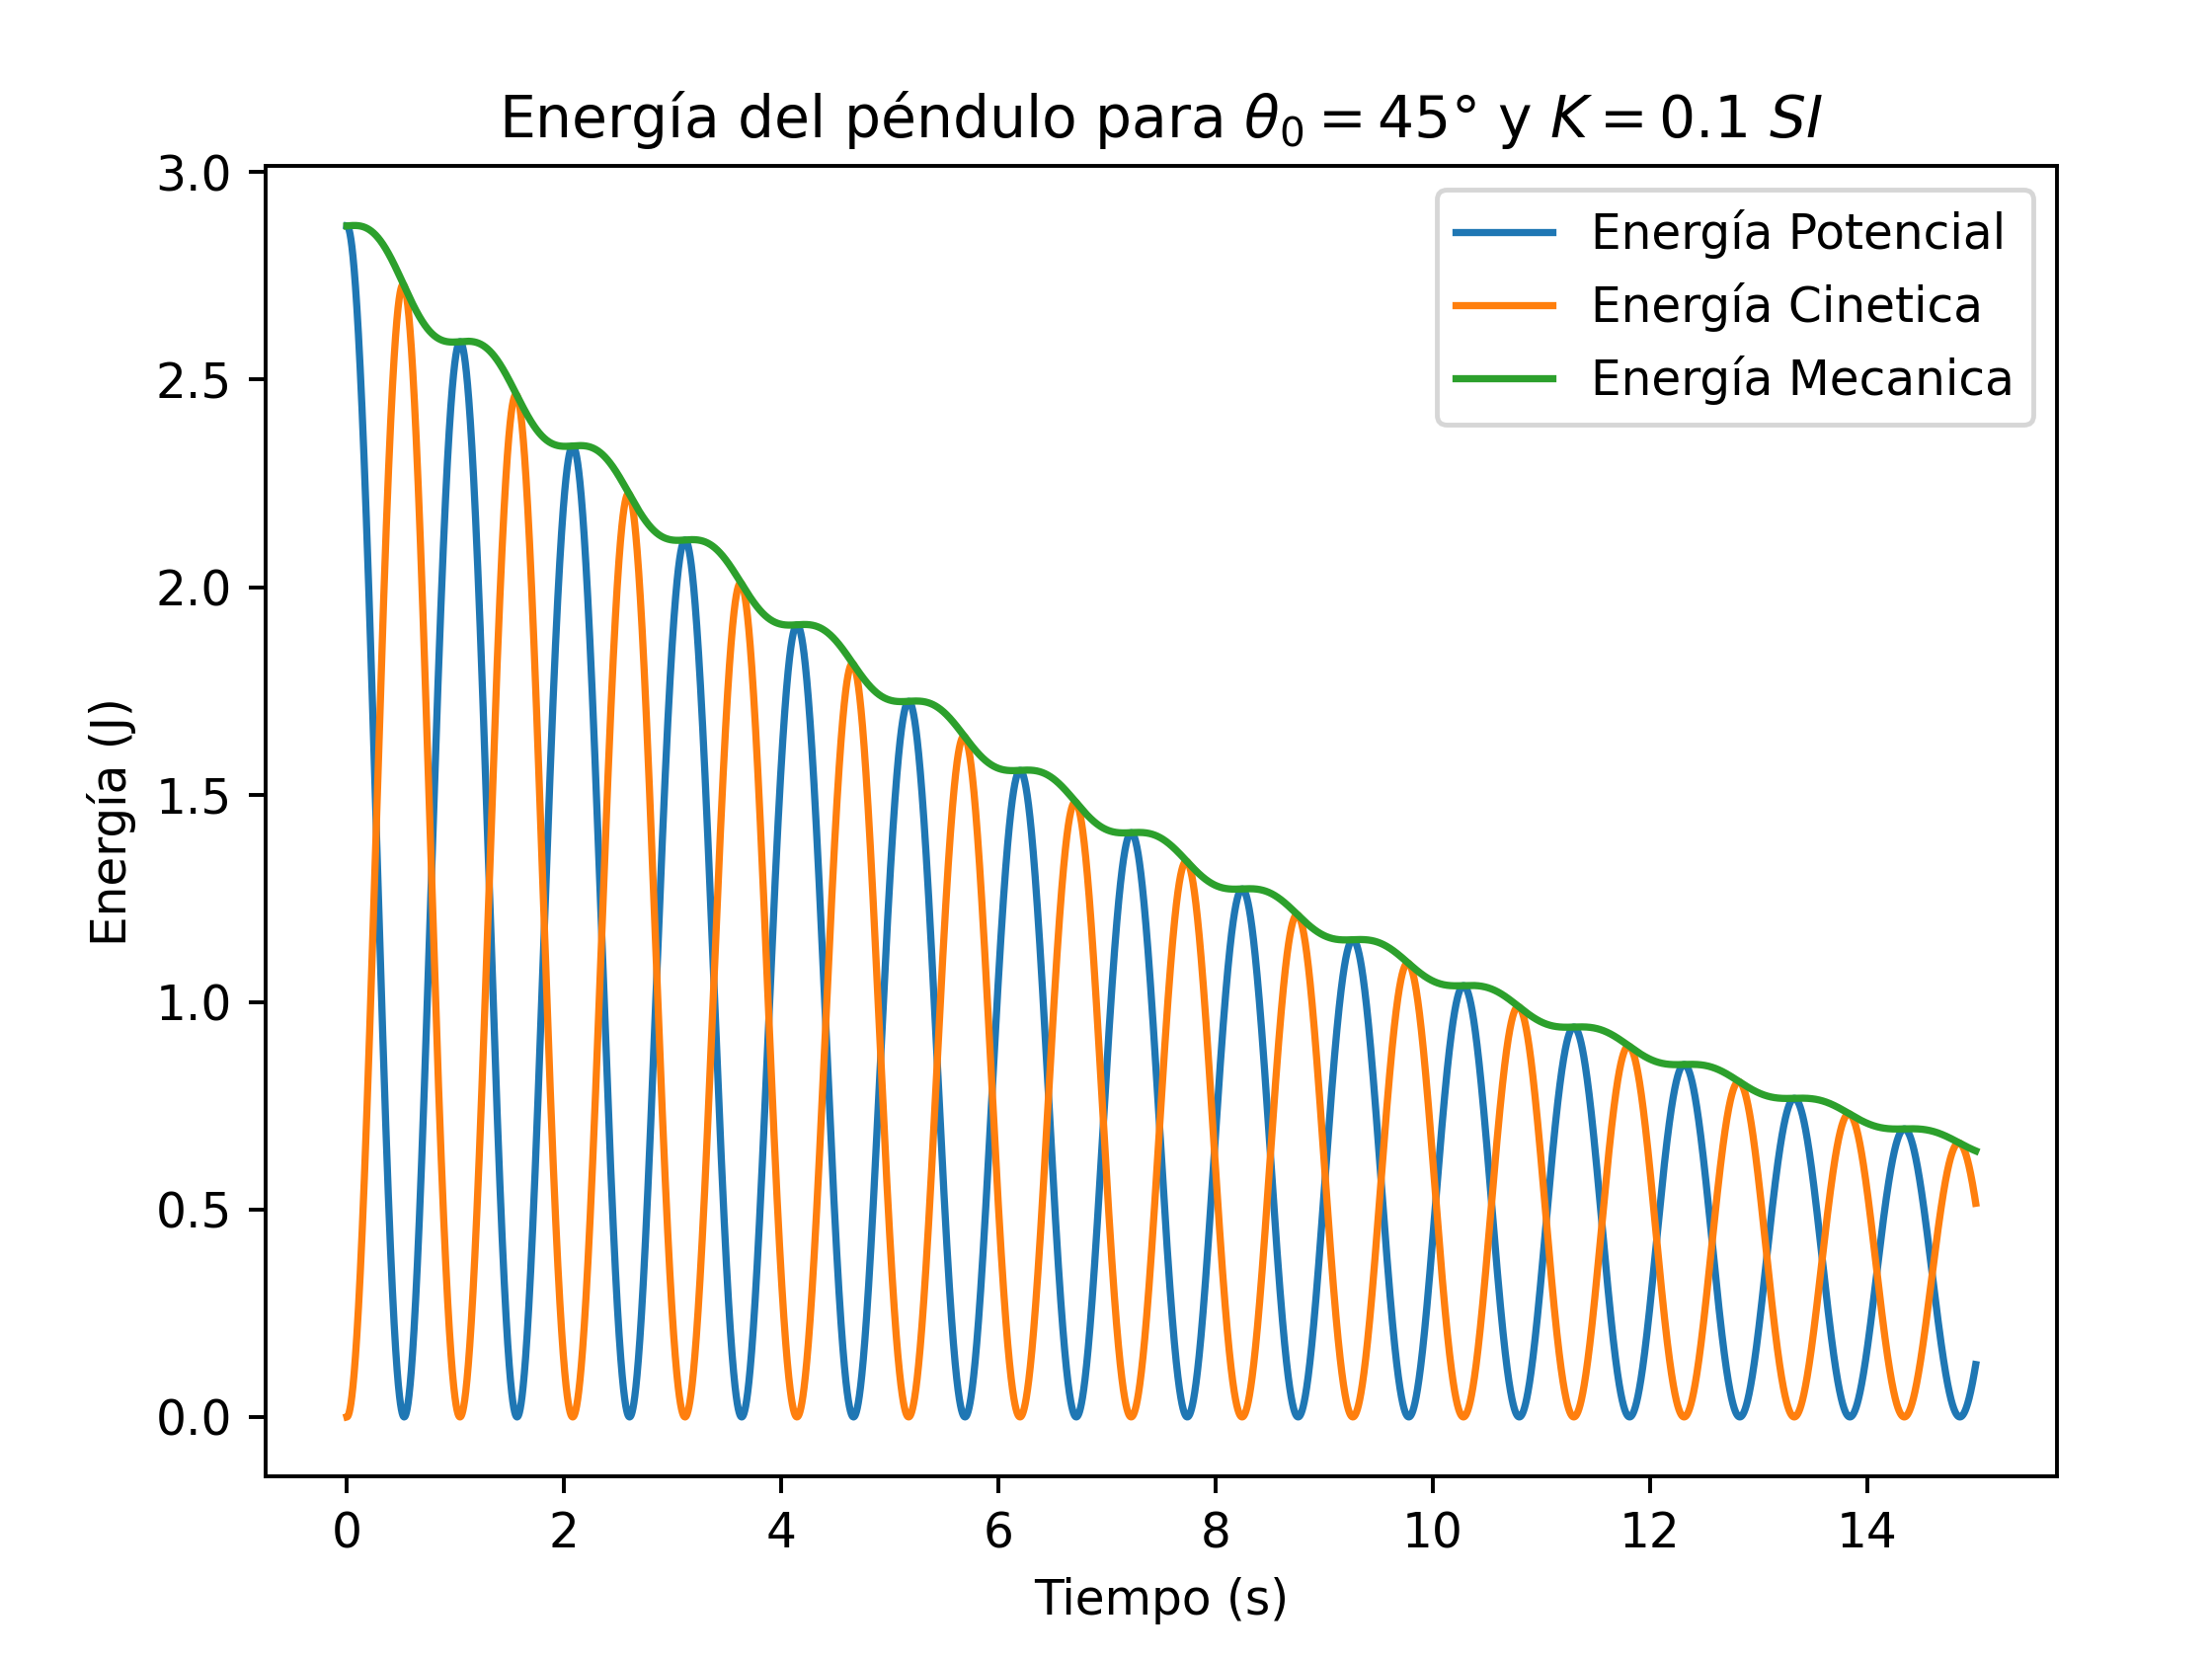
\includegraphics[width=.55\textwidth]{fotos/Fig9.png}
\end{wrapfigure}
\hfill \break \\\\
Sin embargo en esta otra gráfica sí que se ha tenido en cuenta el rozamiento, y podemos comprobar como la energía cae rápidamente a lo largo del tiempo. Esto sucede ya que hemos incluido una fuerza disipatoria, la fuerza de rozamiento. Esto no quiere decir que la energía no se conserve, sino que la energía que en la gráfica anterior siempre estaba en el péndulo como cinética o potencial, ahora poco a poco va convirtiéndose en calor y disipándose al aire mientras roza con él. \\\\ Es interesante observar que el descenso de la energía mecánica no es una curva suave, si no que tiene una forma casi ondulatoria. Esto se debe a que la energía mecánica se disipará en mayor medida cuanto más rápido vaya el péndulo, es decir cuanto mayor sea la energía cinética. Cuando el péndulo alcanza uno de los extremos, la energía cinética será 0, y por tanto no habrá disipación. Es en estos instantes donde la energía mecánica será plana y no descenderá, lo que hace que observemos estos picos en la gráfica.
\end{figure}

\pagebreak
\subsection{Código en python - Anexo 3}
Python es una herramienta muy potente para hacer cálculos de este tipo.Por ejemplo nos permite obtener valores para la varianza de una forma mucho más fácil (una vez escrito el código necesario). \\\\ Aquí se encuentra un código fácilmente reutilizable para otros propósitos, que ajusta los errores de las medidas además de los valores a las cifras significativas de su respectivo error. No solo eso, sino que calcula la varianza y por tanto el error estadístico. Pidiendo el error de interacción y el del instrumento consigue dar un valor para el periodo con su error ajustado una vez se le ha introducido una columna con las medidas. \\\\ Para el caso de la gravedad, tiene programada la relación entre el periodo, la longitud del hilo y la aceleración gravitatoria, con lo que, dándole además del periodo calculado previamente, una longitud del hilo con su error, calcula la aceleración gravitatoria asociada a la columna de datos primeramente introducida. \\\\ Básicamente es un código que calcula todo lo realizado en esta práctica de una forma prácticamente instantánea. De aquí surgen las capturas de consola que han aparecido a lo largo del informe.  
\begin{adjustwidth}{-35pt}{-35pt}
\UseRawInputEncoding
\lstinputlisting[language=Python, firstline=1, lastline=97]{varianzaymedia.py}
\end{adjustwidth}

\end{document}